% Options for packages loaded elsewhere
\PassOptionsToPackage{unicode}{hyperref}
\PassOptionsToPackage{hyphens}{url}
%
\documentclass[
]{article}
\usepackage{amsmath,amssymb}
\usepackage{lmodern}
\usepackage{ifxetex,ifluatex}
\ifnum 0\ifxetex 1\fi\ifluatex 1\fi=0 % if pdftex
  \usepackage[T1]{fontenc}
  \usepackage[utf8]{inputenc}
  \usepackage{textcomp} % provide euro and other symbols
\else % if luatex or xetex
  \usepackage{unicode-math}
  \defaultfontfeatures{Scale=MatchLowercase}
  \defaultfontfeatures[\rmfamily]{Ligatures=TeX,Scale=1}
\fi
% Use upquote if available, for straight quotes in verbatim environments
\IfFileExists{upquote.sty}{\usepackage{upquote}}{}
\IfFileExists{microtype.sty}{% use microtype if available
  \usepackage[]{microtype}
  \UseMicrotypeSet[protrusion]{basicmath} % disable protrusion for tt fonts
}{}
\makeatletter
\@ifundefined{KOMAClassName}{% if non-KOMA class
  \IfFileExists{parskip.sty}{%
    \usepackage{parskip}
  }{% else
    \setlength{\parindent}{0pt}
    \setlength{\parskip}{6pt plus 2pt minus 1pt}}
}{% if KOMA class
  \KOMAoptions{parskip=half}}
\makeatother
\usepackage{xcolor}
\IfFileExists{xurl.sty}{\usepackage{xurl}}{} % add URL line breaks if available
\IfFileExists{bookmark.sty}{\usepackage{bookmark}}{\usepackage{hyperref}}
\hypersetup{
  hidelinks,
  pdfcreator={LaTeX via pandoc}}
\urlstyle{same} % disable monospaced font for URLs
\usepackage[margin=1in]{geometry}
\usepackage{graphicx}
\makeatletter
\def\maxwidth{\ifdim\Gin@nat@width>\linewidth\linewidth\else\Gin@nat@width\fi}
\def\maxheight{\ifdim\Gin@nat@height>\textheight\textheight\else\Gin@nat@height\fi}
\makeatother
% Scale images if necessary, so that they will not overflow the page
% margins by default, and it is still possible to overwrite the defaults
% using explicit options in \includegraphics[width, height, ...]{}
\setkeys{Gin}{width=\maxwidth,height=\maxheight,keepaspectratio}
% Set default figure placement to htbp
\makeatletter
\def\fps@figure{htbp}
\makeatother
\setlength{\emergencystretch}{3em} % prevent overfull lines
\providecommand{\tightlist}{%
  \setlength{\itemsep}{0pt}\setlength{\parskip}{0pt}}
\setcounter{secnumdepth}{-\maxdimen} % remove section numbering
\ifluatex
  \usepackage{selnolig}  % disable illegal ligatures
\fi

\author{}
\date{\vspace{-2.5em}}

\begin{document}

\hypertarget{insured-analysis}{%
\section{Insured-Analysis}\label{insured-analysis}}

The code is avaible in the \texttt{lol.R} file.

With a series of data which correspond to the claims of an insurer in
Monterrey. It is to analyze and combine the risks of the insurer's
portfolio. This report is created as a support for the risk committee to
know the influence of the claims with the variables that are known.

The first step is to take a look at our data.

\begin{verbatim}
#>   Kilometres Zone Bonus Make Insured Claims Payment
#> 1          1    1     1    1  455.13    108  392491
#> 2          1    1     1    2   69.17     19   46221
#> 3          1    1     1    3   72.88     13   15694
#> 4          1    1     1    4 1292.39    124  422201
#> 5          1    1     1    5  191.01     40  119373
#> 6          1    1     1    6  477.66     57  170913
\end{verbatim}

\begin{itemize}
\item
  The kilometers variable describes the category of the number of
  kilometers driven per insured. 1.- \textless1,000 km. 2.- 1,000
  -15,000 km. 3.- 15,000 - 20,000 km. 4.- 20,000 - 25,000 km. 5.- 25,000
  km.
\item
  The zone variable describes the municipality to which the insured
  belongs. 1.- Monterrey. 2.- San Pedro. 3.- San Nicolas. 4.- Escobedo.
  5.- Guadalupe. 6.- Garcia. 7.- Others.
\item
  Variable Bonus: Number of years since the insured filed a claim +1
\item
  Variable Make: Model of the insured car 1-8 represents a certain model
  and 9 represents the rest.
\item
  Insured variable: Number of insured per policy year.
\item
  Claims variable: Number of claims made by the lot or insured.
\end{itemize}

In order to easily observe our data, a descriptive analysis of the
variables is made through histograms.

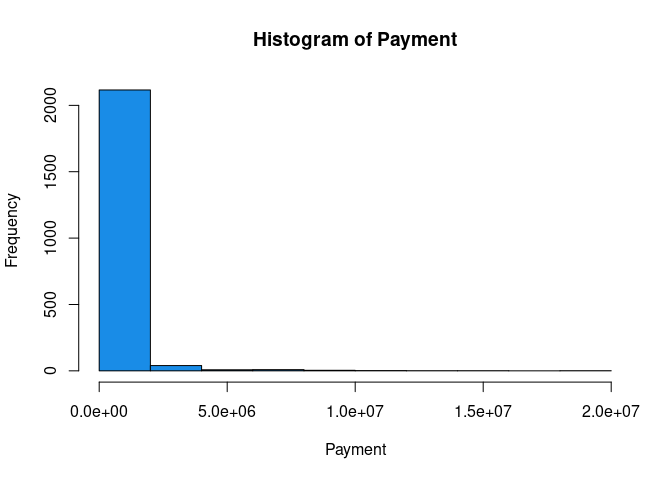
\includegraphics{README_files/figure-latex/pressure-1.pdf}
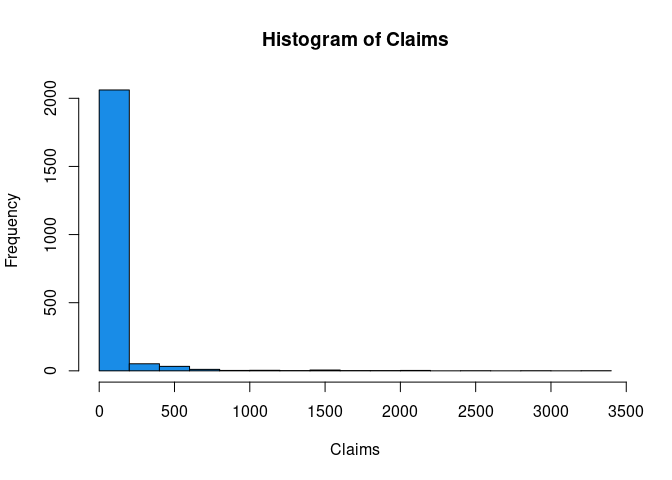
\includegraphics{README_files/figure-latex/pressure-2.pdf}
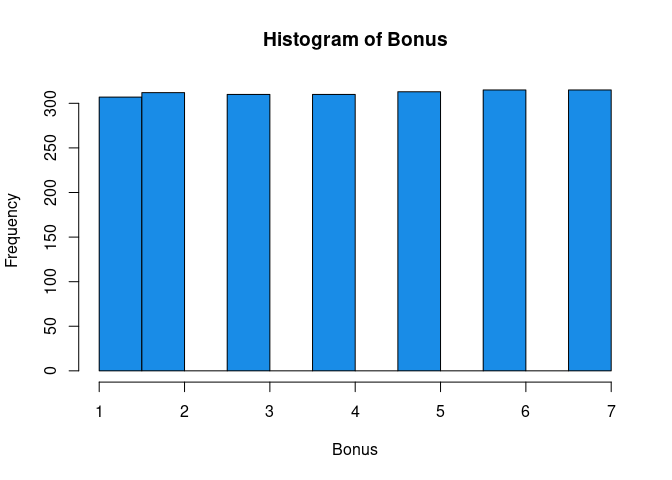
\includegraphics{README_files/figure-latex/pressure-3.pdf}
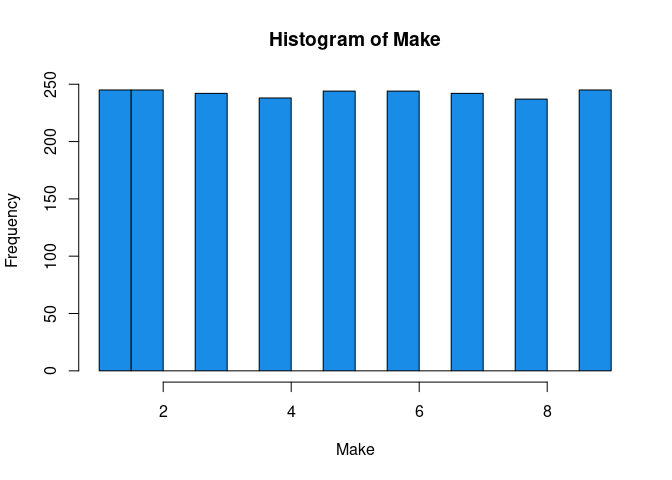
\includegraphics{README_files/figure-latex/pressure-4.pdf}
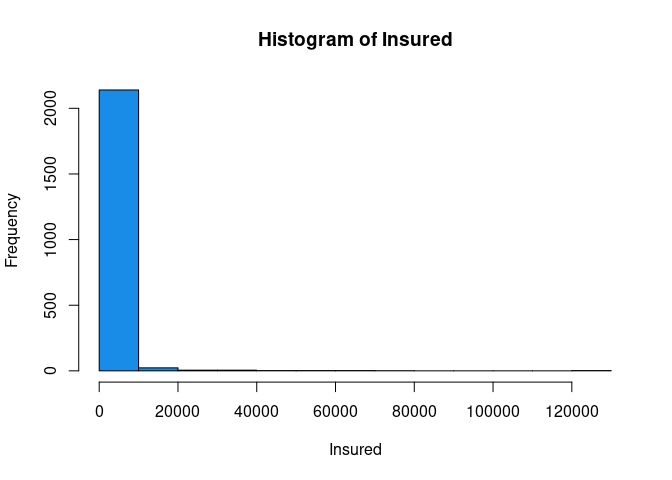
\includegraphics{README_files/figure-latex/pressure-5.pdf}
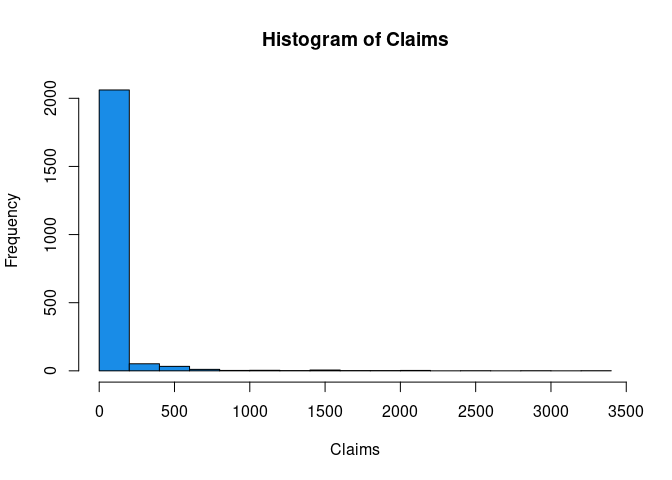
\includegraphics{README_files/figure-latex/pressure-6.pdf}
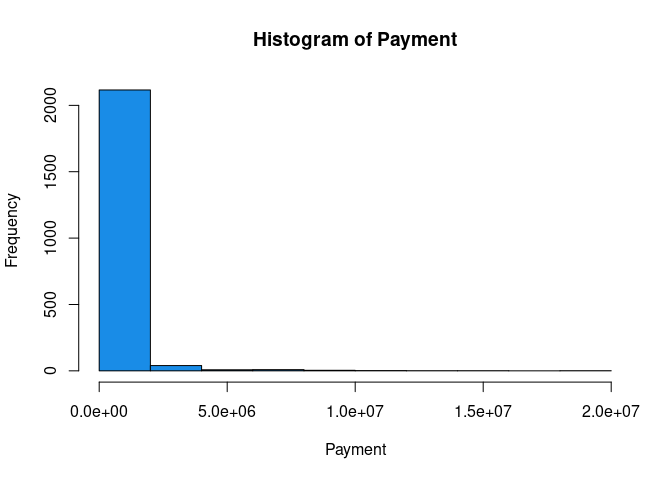
\includegraphics{README_files/figure-latex/pressure-7.pdf}

To have a clear idea of the correlation between all the variables in
terms of kilometers, municipality and model. The following graphs were
made.

\hypertarget{asum-of-insured-per-kilometer}{%
\paragraph{a)Sum of insured per
kilometer:}\label{asum-of-insured-per-kilometer}}

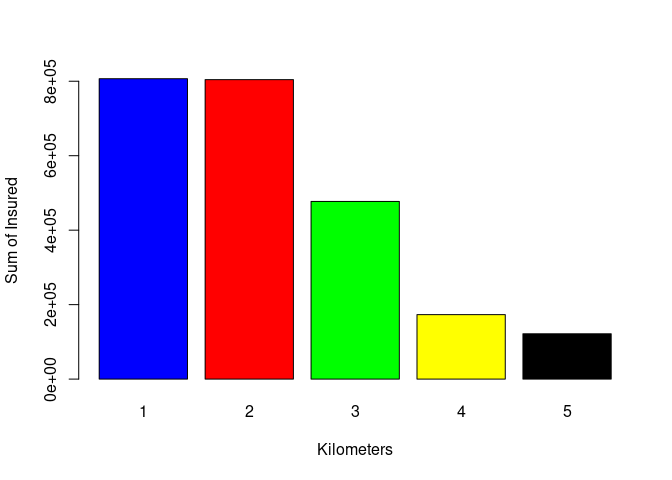
\includegraphics{README_files/figure-latex/unnamed-chunk-4-1.pdf}

\hypertarget{bsum-of-claims-per-kilometer}{%
\paragraph{b)Sum of claims per
kilometer:}\label{bsum-of-claims-per-kilometer}}

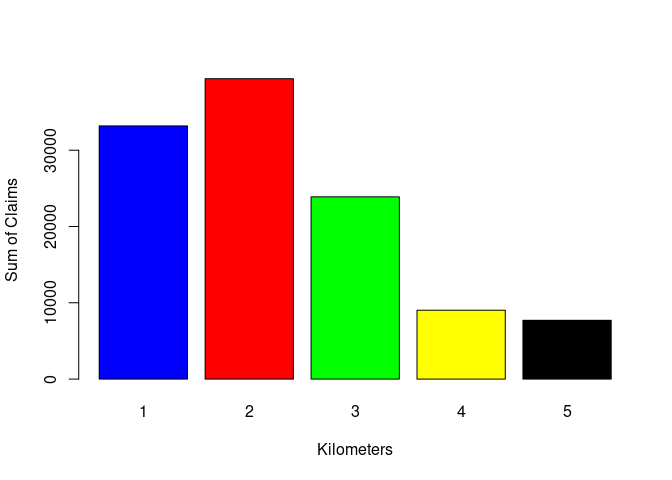
\includegraphics{README_files/figure-latex/unnamed-chunk-5-1.pdf}

\hypertarget{csum-of-pays-per-kilometer}{%
\paragraph{c)Sum of pays per
kilometer:}\label{csum-of-pays-per-kilometer}}

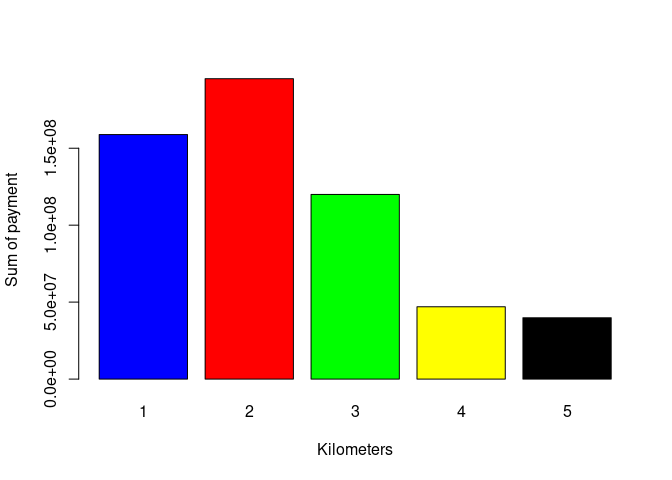
\includegraphics{README_files/figure-latex/unnamed-chunk-6-1.pdf}

We can see in the graphs that a similar trend is followed in the 3 cases
for the relationship between the variables we are using with the
kilometers variable.

\hypertarget{dsum-of-claims-per-zone}{%
\paragraph{d)Sum of claims per Zone:}\label{dsum-of-claims-per-zone}}

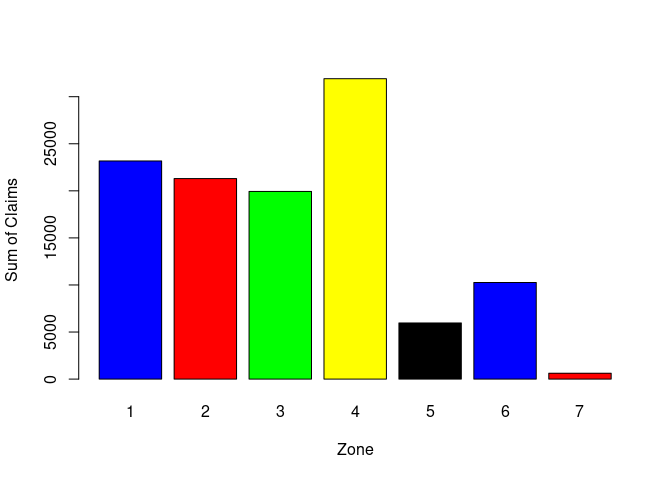
\includegraphics{README_files/figure-latex/unnamed-chunk-7-1.pdf}

\hypertarget{esum-of-insured-per-zone}{%
\paragraph{e)Sum of Insured per Zone:}\label{esum-of-insured-per-zone}}

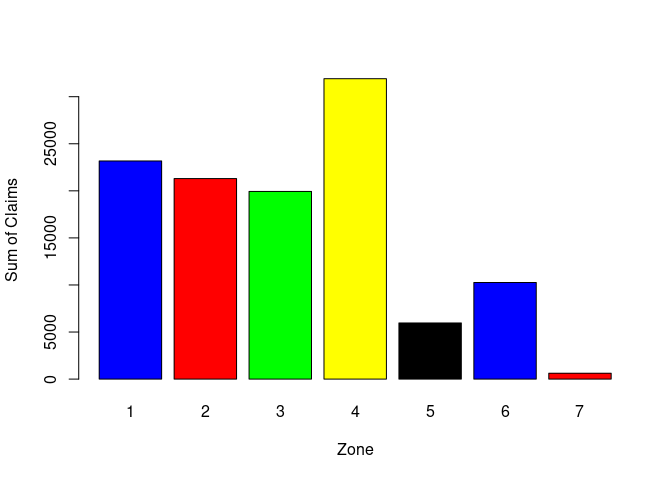
\includegraphics{README_files/figure-latex/unnamed-chunk-8-1.pdf}

\hypertarget{fsum-of-payments-per-zone}{%
\paragraph{f)Sum of payments per
Zone:}\label{fsum-of-payments-per-zone}}

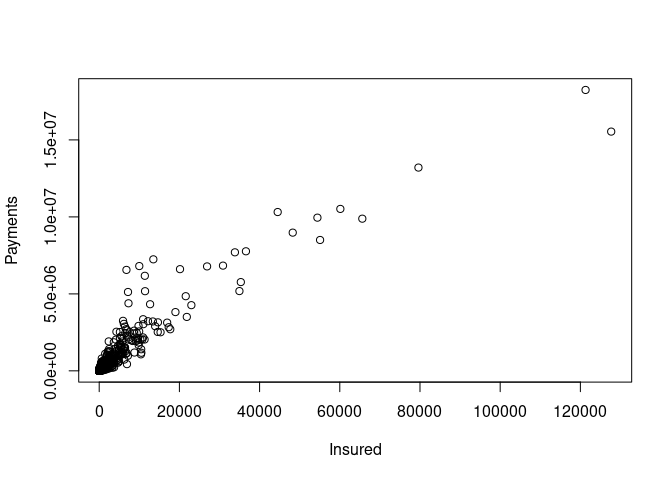
\includegraphics{README_files/figure-latex/unnamed-chunk-9-1.pdf}

\hypertarget{gsum-of-claims-per-model}{%
\paragraph{g)Sum of claims per Model:}\label{gsum-of-claims-per-model}}

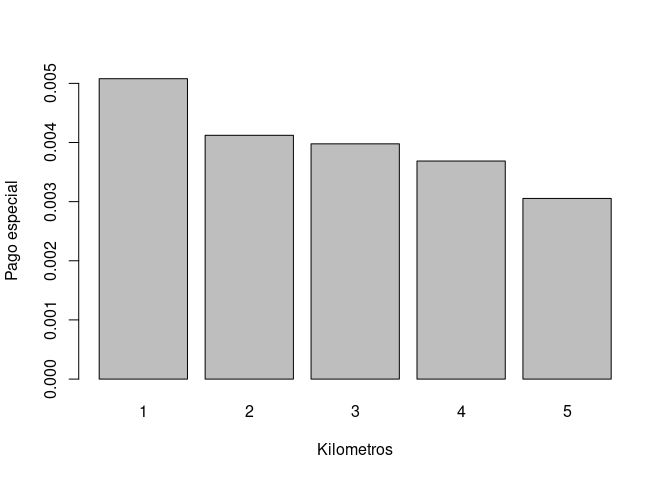
\includegraphics{README_files/figure-latex/unnamed-chunk-10-1.pdf}

\hypertarget{hsum-of-insured-per-model}{%
\paragraph{h)Sum of Insured per
Model:}\label{hsum-of-insured-per-model}}

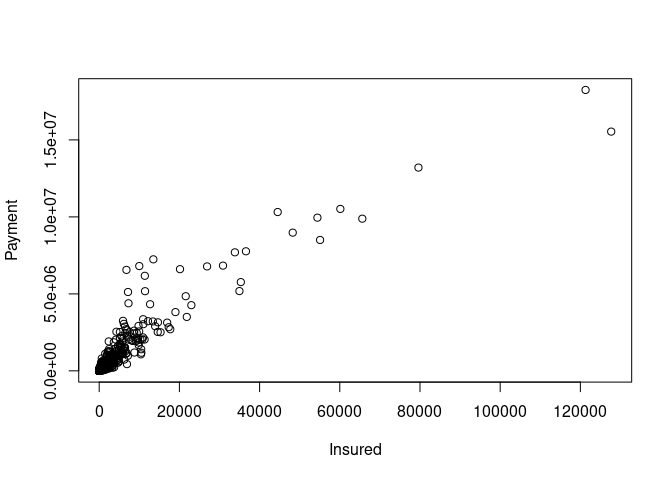
\includegraphics{README_files/figure-latex/unnamed-chunk-11-1.pdf}

\hypertarget{gsum-of-payments-per-model}{%
\paragraph{g)Sum of Payments per
Model:}\label{gsum-of-payments-per-model}}

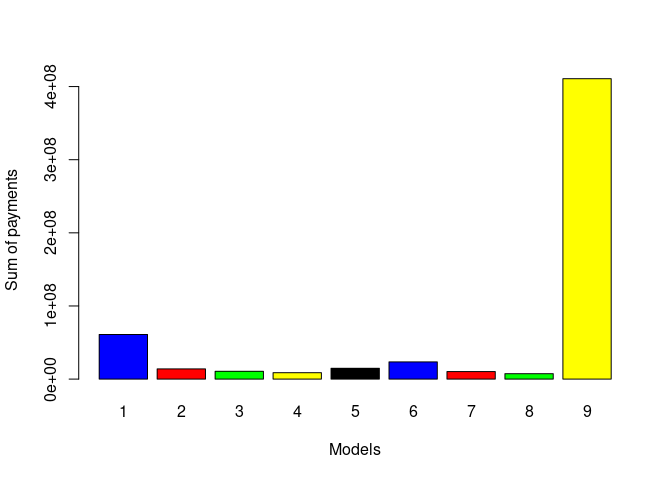
\includegraphics{README_files/figure-latex/unnamed-chunk-12-1.pdf}

\end{document}
